\subsection{Total Variation(TV) Based Applications}
\label{subsec:TV Applications}

%Total variation(TV) For a function$f(x)$ defined on a domain $\Omega\subseteq\mathbb{R}^n$, its TV is defined as
%
%\small{
%\begin{equation}
% \label{eq:continuousTV1}
% J_{f}=\int_{\Omega}^{}| \nabla f |dx,
%\end{equation}
%}
%\\
%where $| \nabla f |$ is the $\ell_2$-norm of the gradient $\nabla f$, i.e.,
%
%\small{
%\begin{equation}
% \label{eq:continuousTV2}
% | \nabla f |= \sqrt{ \sum_{i=1}^{} ( \frac{\partial f} {\partial x_{i}} )^2}.
%\end{equation}
%}
%\\

Total variation(TV) has been a popular tool for image processing tasks,such as denoising, reconstruction, and segmentation\cite{chambolle2010introduction}.
the underlying model for TV methods aims at exploiting the sparsity of the gradient of image pixel values.
The discrete variant yields the following convex objective function

\small{
\begin{equation}
 \label{eq:descreteTV}
 TV(\mathbf{u})=\sum_{i,j}^{}\|\mathcal{D}_{i,j} \mathbf{u}\|_2
\end{equation}
}
\\
where $\mathcal{D}_{i,j}$ is the discrete gradient operator at pixel $(i,j)$ and $\mathbf{u}$ is a vector containing the gray-level pixel values. TV methods filter the image by minimizing TV$(\mathbf{u})$ which is in fact the $\ell_1$ norm of the vector $[\cdots~\|\mathcal{D}_{i,j}\mathbf{u}\|_2~\cdots]$.
Since TV is designed for images, it is not directly applicable to geometry processing problem.
As we have stated, the key point is to find some form of second order information.

Note that some of the following applications have been reviewed in previous sections, but considering the good development of TV in geometry processing, we take one subsection to introduce its applications attempting to help readers understands it better.

\subsubsection{Point cloud consolidation}
\label{subsubsec:TVPoint cloud consolidation}

In section~\ref{subsec:Point Cloud Consolidation}, the consolidation works are all $\ell_1$ median based.
Here we review one more well-known work.
Similar to the sparse gradient minimization, and based on the observation that the gradients(normal differences) of smooth surface normals(normal differences) are sparse,
\cite{avron2010L1} formulates the piecewise smoothness reconstruction problem as a sparse minimization of orientation differences and position projections as following

\small{
\begin{equation}
 \label{eq:TVconsolidation1}
 \begin{aligned}
 &N^{out} =\mathop{\argmin}_{N} \sum_{(p_{i},p_{j})\in E}^{} w_{i,j}\|n_{i}-n_{j}\|_2\\
 &\mathrm{s.t.}~\forall i~\|n_{i}-{n_{i}}^{in}\|_2\le \gamma_{n}
 \end{aligned}
\end{equation}
}
\small{
\begin{equation}
 \label{eq:TVconsolidation2}
 X^{out} = \mathop{\argmin}_{X} \sum_{(p_{i},p_{j})\in E}^{} w_{i,j}|n_{i,j}\cdot (x_{i}-x_{j})|
\end{equation}
}
\\
where $\{n_{i}\}$ denote the surface normals, $\{x_{i}\}$ denote the point positions and $\{w_{i,j}\}$ is a set of the weight whose role is to achieve lower-than-$\ell_1$ sparsity.

Convexity of these two problems allows for finding a global optimum and deriving efficient solvers.
Figure~\ref{fig:TV consolidation} shows a well reconstructed example with sharp features.
Due to the global nature, this algorithm is extremely slow.
And it may fail for the point set with severe noises and outliers.

\begin{figure}[ht]
  \centering
  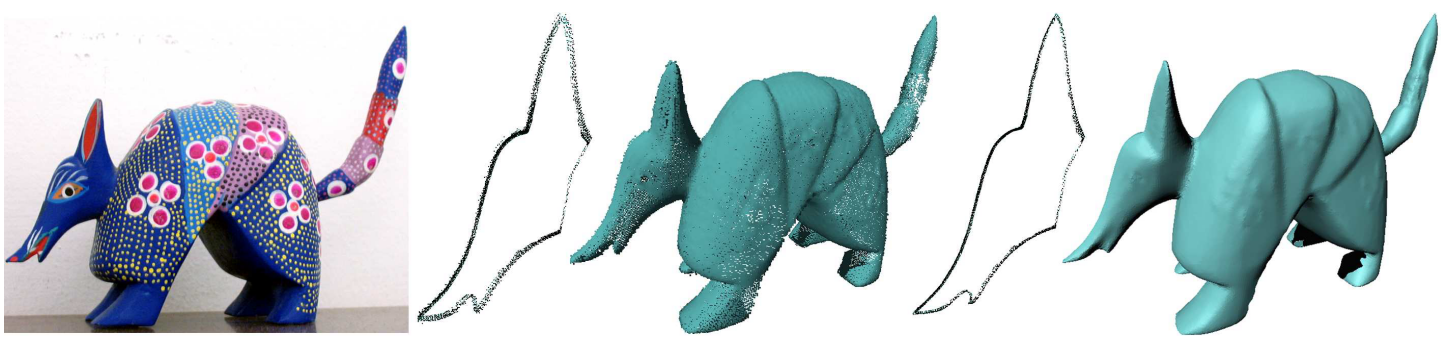
\includegraphics[width=3in]{images/TV_consolidation}
  \caption{Sparse regularization: TV based point cloud consolidation\cite{lipman2007parameterization}. The Armadillo statue(left) is scanned generating a noisy point-cloud(middle). The right figure shows the consolidation result preserving the sharp features.}
  \label{fig:TV consolidation}
\end{figure}


\subsubsection{Mesh Denoising}
\label{subsubsec:mesh denoising}
Unlike\cite{he2013mesh} achieving denoising with a new proposed edge operator, \cite{zhang2014variational}, adopting the sparsity of face normals differences, proposes a two-phase method including $face$ normal filtering and vertex updating.
They filter face normals with a new variational denoising method based on the definition of piecewise constant function spaces and associated differential operators on triangulated surfaces.

\paragraph{Piecewise constant function spaces and operators}
For a space $V_{M}=\mathbb{R}^{T}$ equipped with well-defined inner product and norm, it is isomorphic to the piecewise constant function space over surface $M$, i.e., $u=(u_0,u_1,\cdots, u_{T-1})\in V_{M}$, $T$ is the triangle number in $M$ and $u_{\tau}$ denotes the value of $u$ restricted on the triangle $\tau$. After defining the jump of $u\in V_{M}$ over an edge $e$ as

\small{
\begin{equation}
 \label{eq:edgejump}
 [u]_{e} := \left \{
 \begin{aligned}
 & \sum_{e\prec\tau}^{} u|_{\tau} \textrm{sgn}(e, \tau),  &e\nsubseteq \partial M \\
 & 0,  &e\subseteq \partial M
 \end{aligned}
 \right.
\end{equation}
}
\\
the gradient operator is defined as
\small{
\begin{equation}
 \label{eq:edgegradient}
 \nabla:u\rightarrow \nabla u, \nabla u|_{e}=[u]_{e},~\forall e, ~\textrm{for}~u\in V_{M}.
\end{equation}
}
\\
here, $e\prec\tau$ indicates that $e$ is an edge of the triangle $\tau$, then if the orientation of $e$ is consistent with the orientation of $\tau$, $\textrm{sgn}(e, \tau)=1$; otherwise $\textrm{sgn}(e, \tau)$=-1.

Due to the ambiguity of the tangent space at an edge, they define another space $Q_{M}=\textrm{Range}(\nabla)$. The divergence operator, div: $Q_{M}\rightarrow V_{M}$, as the adjoint operator of $-\nabla$, is formulated as

\small{
\begin{equation}
 \label{eq:edgedivergence}
 (\textrm{div}p|_{\tau})=\frac{-1}{s_{\tau}}
 \sum_{e\prec\tau,e\nsubseteq \partial M}^{}
 l_{e} p|_{e} \textrm{sgn}(e, \tau),~\forall p\in Q_{M}.
\end{equation}
}
\\
where, $s_{\tau}$ is the area of triangle $\tau$, $l_{e}$ is the length of edge $e$.
Thus for $u\in V_{M}$, the total variation is

\small{
\begin{equation}
 \label{eq:elementtv}
 R_{\textrm{tv}}(\nabla u) = (\textrm{TV})(u)
 = \sum_{e}^{} l_{e} | (\nabla u)|_{e} |
 = \sum_{e}^{} l_{e} | [u]_{e} |.
\end{equation}
}
\\
here, $l_{e}$ just meets the perimeter formulae defined using total variation of the characteristic function. To be more suitable to practical applications, they extend the above definition to vectorial case, for $_{\mathfrak{N}}$-channel data

\small{
\begin{equation}
 \label{eq:vectorialspace}
 \mathbf{V}_{M} = \underbrace{V_{M}\times\cdots\times V_{M}}_{\mathfrak{N}},
 \mathbf{Q}_{M} = \underbrace{Q_{M}\times\cdots\times Q_{M}}_{\mathfrak{N}}
\end{equation}
}
\\
and the vectorial total variation of $\mathbf{u}\in\mathbf{V}_M$ is

\small{
\begin{equation}
 \label{eq:vectorialtv}
  R_{\textrm{vtv}}(\nabla \mathbf{u}) = (\textrm{TV})(\mathbf{u})
 = \sum_{e}^{}   \sqrt{\sum_{i=1}^{\mathfrak{N}}  l_{e} | [u_{i}]|_{e} |^2} .
\end{equation}
}

\paragraph{Variational model}
Based on these definitions, they give a new variational face normals($\mathbf{N}$) filtering method formulated as

\small{
\begin{equation}
 \label{eq:denoisingmodeltv1}
 \min_{\mathbf{N}\in C_{\mathbf{N}}}
 \left\{
 R_{\textrm{wvtv}}(\nabla \mathbf{N})+
 \frac{\alpha}{2} \| \mathbf{N}-\mathbf{N}^{in} \|{_{\mathbf{V}_M}^{2}}
 \right\},
\end{equation}
}
\\
where
\small{
\begin{equation}
 \label{eq:denoisingmodeltv2}
 \begin{aligned}
 & R_{\textrm{wvtv}}(\nabla \mathbf{N})
 = \sum_{e}^{} w_{e}   \sqrt{\sum_{i=1}^{3}  l_{e} | [N_{i}]|_{e} |^2},\\
 & C_{\mathbf{N}}=\left\{ \mathbf{N}\in\mathbf{V}_M: \| \mathbf{N}_{\tau} \|_2=1,~\forall\tau  \right\}
 \end{aligned}
\end{equation}
}
\\
with $w_{e}$ as a weight aiming for improving preserving sharp features.
Iteratively solving this variational model~(\ref{eq:denoisingmodeltv1}) and updating vertex using previous method, the denoising results preserving sharp features can be obtained as shown in Figure~\ref{fig:denoise_tv}.
Like many other optimization problem, the optimal values of the parameters, like $\alpha$, are given by the experimental data and there is of course no theoretical convergence guarantee.

\begin{figure}[ht]
  \centering
  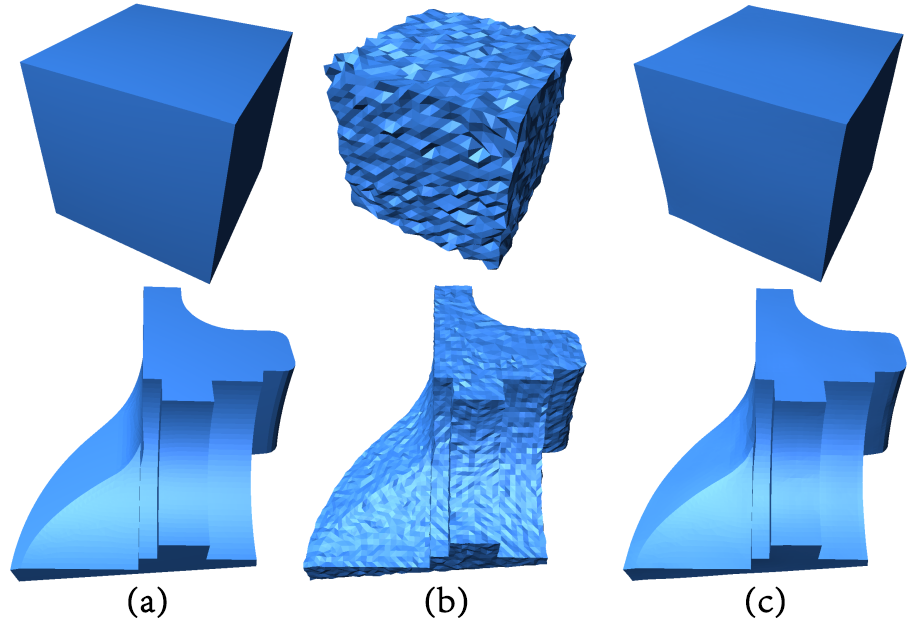
\includegraphics[width=2.5in]{images/denoise_tv}
  \caption{Sparse regularization: TV based mesh denoising\cite{zhang2014variational}. (a): clean meshes. (b): noisy mesh(Gaussian noise, standard deviation=0.2 mean edge length for Cube; standard deviation=0.1 mean edge length for Fandisk). (c): denoising result.}
  \label{fig:denoise_tv}
\end{figure}


\subsubsection{Decomposition}
\label{subsubsection:Decompsition}

Mesh decomposition means segmenting a mesh into meaningful parts that are consistent with user intention, geometric mesh attributes, and human shape perception.
Generally, the elements within the same segment should have high similarity, the segment boundary should be tight and smooth as well as matching human perception, and obviously the segmentation should reflect significant features.

Motivated by the preceding observation, \cite{zhang2012variational} proposes a new method based on the Mumford-Shah model(M-S model)\cite{mumford1989optimal} that has proven successful in image segmentation, i.e., this method is also an extension from 2D images to 3D meshes.

In 2D image $I:\Omega\rightarrow \mathbb{R}^2$, the Mumford-Shah image segmentation is to find a partition $\Omega=\bigcup{_{i=1}^{k}}\Omega_{i}$, where $\Omega_{i}$ are pairwise disjoint, and numbers $c_{i}$ for $\Omega_{i}$ formulated as

\small{
\begin{equation}
 \label{eq:TV image M-S}
 \inf_{\Omega_{i},c_{i}} \sum_{}^{k}
 ( \int_{\Omega_{i}}^{} (I(x)-c_{i})^2dx + \frac{\mu}{2} | \partial\Omega_{i} | ),
\end{equation}
}
\\
where $\mu$ is a constant, $\partial \Omega$ and $|\partial \Omega|$ represent the boundary and the boundary length of segment $\Omega$, respectively.
The first data term measures the consistency of each segment and the second regularization term measures the boundary length.

To segment a 3D triangulated surface $M$, \cite{zhang2012variational} convexifies this difficult nonconvex problem~(\ref{eq:TV image M-S}) based on TV to get a new version of M-S model

\small{
\begin{equation}
 \label{eq:TV surface M-S}
 \min_{\mathbf{u}\in K, \chi_{i}} \left \{
 \int_{M}\langle\mathbf{u}(x), \mathbf{s}(x)\rangle +
 \mu g(x)| \nabla_{M}\mathbf{u}(x) | d\sigma
 \right\},
\end{equation}
}
\\
where $K$ is the set of vector functions $\mathbf{u}=(u_1,\cdots,u_{k})^{T}:M\rightarrow \mathbb{R}^{k}$ satisfying that for all $x\in M$ and $i\in [1,\cdots,k],u_{i}(x)\geq0$ and
$\sum_{i=1}^{k}u_{i}(x)=1; \mathbf{s}(x)=(s_1(x),\cdots,s_k(x))^T$ is a $k$-dimensional vector with $s_i(x)=(\mathbf{f}(x)-\chi_{i})^{T}(\mathbf{f}(x)-\chi_{i})$ indicating
the affinity vector $\chi_{i}$ that is associated with $M_{i}$ which is a segment.
The $\mathbf{f}(x)$ is constructed with the eigenvectors of the Laplacian matrix of the dual graph of $M$ to represent some attributions of $x$ over mesh $M$ similar to the RGB function for an image.
Since the regularization term is to constrain the boundary with some geometric difference information between segments, this optimization may fail for the relative smooth models.

In~(\ref{eq:TV surface M-S}), if the affinity of $x$ with segment $M_{i}$ is large, $u_{i}(x)$ will tend to be small in order to reach the minimization,
thus $u_{i}(x)$ can be viewed as the probability of $x$ being assigned to segment $M_{i}$ and
so $\mathbf{u}(x)$ is used as a classification function for the segmentation achieved with some following processing work.
Different kind of segmentation results are shown in Figure~\ref{fig:segmentation}.


\begin{figure}[ht]
  \centering
  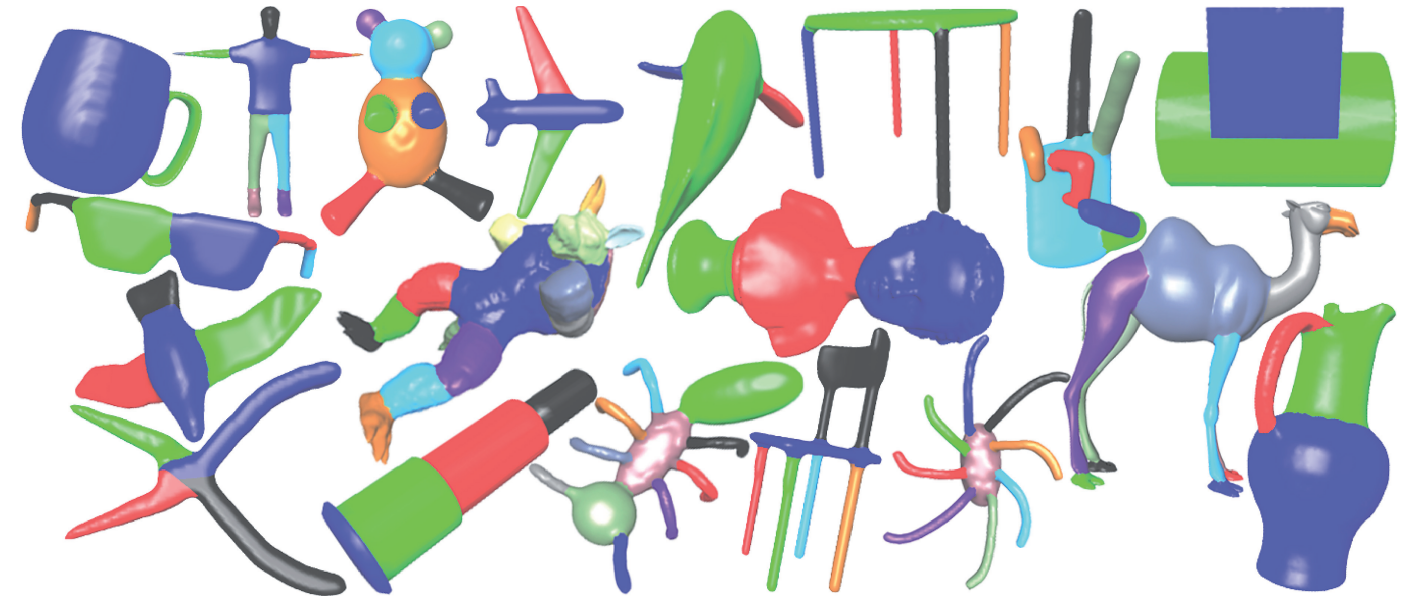
\includegraphics[width=3in]{images/segmentation}
  \caption{Sparse regularization: TV based mesh decomposition\cite{zhang2012variational}. Decomposition results where the models are taken from the Princeton Segmentation Benchmark\cite{chen2009benchmark}. One mesh is shown for each category. The segmentation results match results match human perception well in not only the cutting boundaries but also the number of segments.}
  \label{fig:segmentation}
\end{figure}


\subsubsection{Barycentric coordinates}
\label{subsubsec:Barycentric coordinates}

Barycentric~coordinates provide a simple and convenient way of interpolating values from a set of control points over the interior of a domain, using weighted combinations of values associated with different control points.
Many barycentric coordinates typically get a interpolated value depends on many, potentially $all$, control points.
Then locality, scalability, and moderate computation cost can not be achieved.

\cite{zhang2014local} introduces a novel method to derive $local~barycentric~coordinates$(LBC) that depend only on a small number of control points.
Given a set of control points $\mathbf{c}_1, \cdots, \mathbf{c}_n$ in $\mathbb{R}^2$ or  $\mathbb{R}^3$ which are the vertices of a closed control cage that bounds a domain.
The goal is to find a function $w_{i}$: $\Omega\rightarrow\mathbb{R}$ for each $\mathbf{c}_{i}$, such that $[w_1(\mathbf{x}), \cdots, w_n(\mathbf{x})]$ is a set of generalized barycentric coordinates of $\mathbf{x}\in\Omega$ with respect to the control points $\{\mathbf{c}_{i}\}$ and is used for interpolating function values $f(\mathbf{c}_1), \cdots, f(\mathbf{c}_n)$ at control points on the interior of $\Omega$ by

\small{
\begin{equation}
 \label{eq:BC}
 f(\mathbf{x}) = \sum_{i=1}^{n}w_{i}(\mathbf{x})f(\mathbf{c}_{i}),
\end{equation}
}
\\
except for the properties satisfied in many barycentric coordinate schemes, like reproduction and partition of unity,
they prefer a target $convex$ functional that also reflects $locality$ and $smoothness$ for the coordinate functions.

For a function $w_{i}$ and a given value $s$, denote by $\{w_{i}>s\}:=\{\mathbf{x}|w_{i}(\mathbf{x})>s\}$ and $\{w_{i}=s\}:=\{\mathbf{x}|w_{i}(\mathbf{x})=s\}$ the $superlevel~set$ and the $level set$ of $s$, respectively.
Locality requires the area of the superlevel set $\{w_{i}>0\}$ to be small which means that the vector$[w_{1}(\mathbf{x}), \cdots, w_{n}(\mathbf{x})]$ is sparse, while for smoothness it is necessary that all curves/surfaces $w_{i}=\textrm{const}$ are smooth.

Then the locality and smoothness of $w_{i}$ can be obtained using a functional that measures the sum of the perimeters of superlevel sets $\{w_{i}>s\}$ for all $s$.
That is, the perimeter of each superlevel set regularizes the smoothness of its boundary level curve/surface, while the perimeter of $\{w_{i}>0\}$ penalizes the area of the influence region. 
This functional is exactly the total variation of $\{w_{i}\}$ formulated as

\small{
\begin{equation}
 \label{eq:continuousLBC}
 \begin{aligned}
 & \min_{w_1, \cdots, w_2} \sum_{i=1}^{n} \int_{\Omega}^{} |\bigtriangledown w_{i}| \\
 & ~~~\mathrm{s.t.}~ \sum_{i=1}^{n}w_{i}(\mathbf{x})\mathbf{c}_{i}=\mathbf{x},
        \sum_{i=1}^{n}w_{i}=1,~w_{i}\geq0,~\forall \mathbf{x}\in\Omega,\\
 & ~~~~~~~~w_{i}(\mathbf{c}_{j})=\delta_{ij},~forall i,j,\\
 & ~~~~~~~~w_{i}~\textrm{is linear on cage edges and faces }\forall i.
 \end{aligned}
\end{equation}
}
\\
Discretely, after triangulating the domain $\Omega$, each $w_{i}$ is represented a function that is linear within each cell(triangle in 2D or tetrahedron in 3D) and then the gradient of $w_{i}$ is constant on each cell. Let $\mathcal{C}$ be the set of cells in the triangulation, the target functional~(\ref{eq:continuousLBC}) finally becomes

\small{
\begin{equation}
 \label{eq:discreteLBC}
 \sum_{T\in\mathcal{C}}^{}  \sum_{i=1}^{}
 \phi{_{i}^{T}}  A_{T}  \| \nabla T w_{i} \|_2,
\end{equation}
}
\\
where $\nabla T w_{i}$ is the gradient of $w_{i}$ in cell $T$, $A_{T}$ is the area(volume) of $T$, and $\phi{_{i}^{T}}$ is the value of the weighting function $\phi_{i}$ at the centroid of $T$.

Figure~\ref{fig:LBC} shows a cage-based deformation example with lower computational and storage requirement since each point on the target shape is only determined by a small number of control points.
Whatever, from the observation, we can see that there is a trade-off between locality and smoothness which is a common troubling issue for so many existing works.

\begin{figure}[ht]
  \centering
  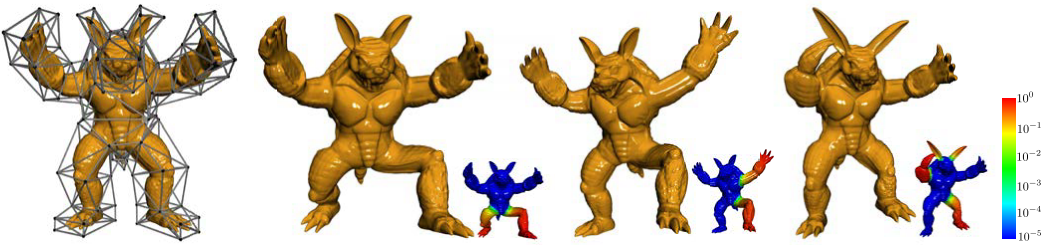
\includegraphics[width=3in]{images/LBC_L1}
  \caption{Sparse regularization: TV based local barycentric coordinates\cite{zhang2014local}. Using LBC for 3D cage-based manipulation allows for local, smooth and shape-aware deformations. Only parts near the manipulated control points are deformed, as indicated by the color-coding.}
  \label{fig:LBC}
\end{figure}
